\chapter{Regimes transitórios: primeira e segunda ordem}\label{ch:b1:transient-regimes}

Aperte o canto de um carro estacionado e solte. Um carro em bom
estado sobe uma vez e para; um carro com amortecedores gastos balança duas ou
três vezes antes de se acomodar. Num laboratório de eletrônica os mesmos dois
comportamentos aparecem num osciloscópio quando um capacitor se descarrega através
de uma bobina: um retorno suave, ou uma oscilação que se extingue. Ambos são o
\emph{transitório} entre um \omterm{def:b1:transient-regimes:firstorder}{regime permanente} e outro, e ambos obedecem
à mesma pequena família de equações diferenciais lineares --- primeira ordem
para um único reservatório de energia, segunda ordem para dois que trocam energia. Este
capítulo as resolve de uma vez por todas, nomeia os seus parâmetros (\omterm{def:b1:transient-regimes:firstorder}{constante
de tempo}, frequência própria, \omterm{def:b1:transient-regimes:secondorder}{fator de qualidade}) e mostra como os mesmos
números descrevem um circuito e uma suspensão.

\begin{omfigure}
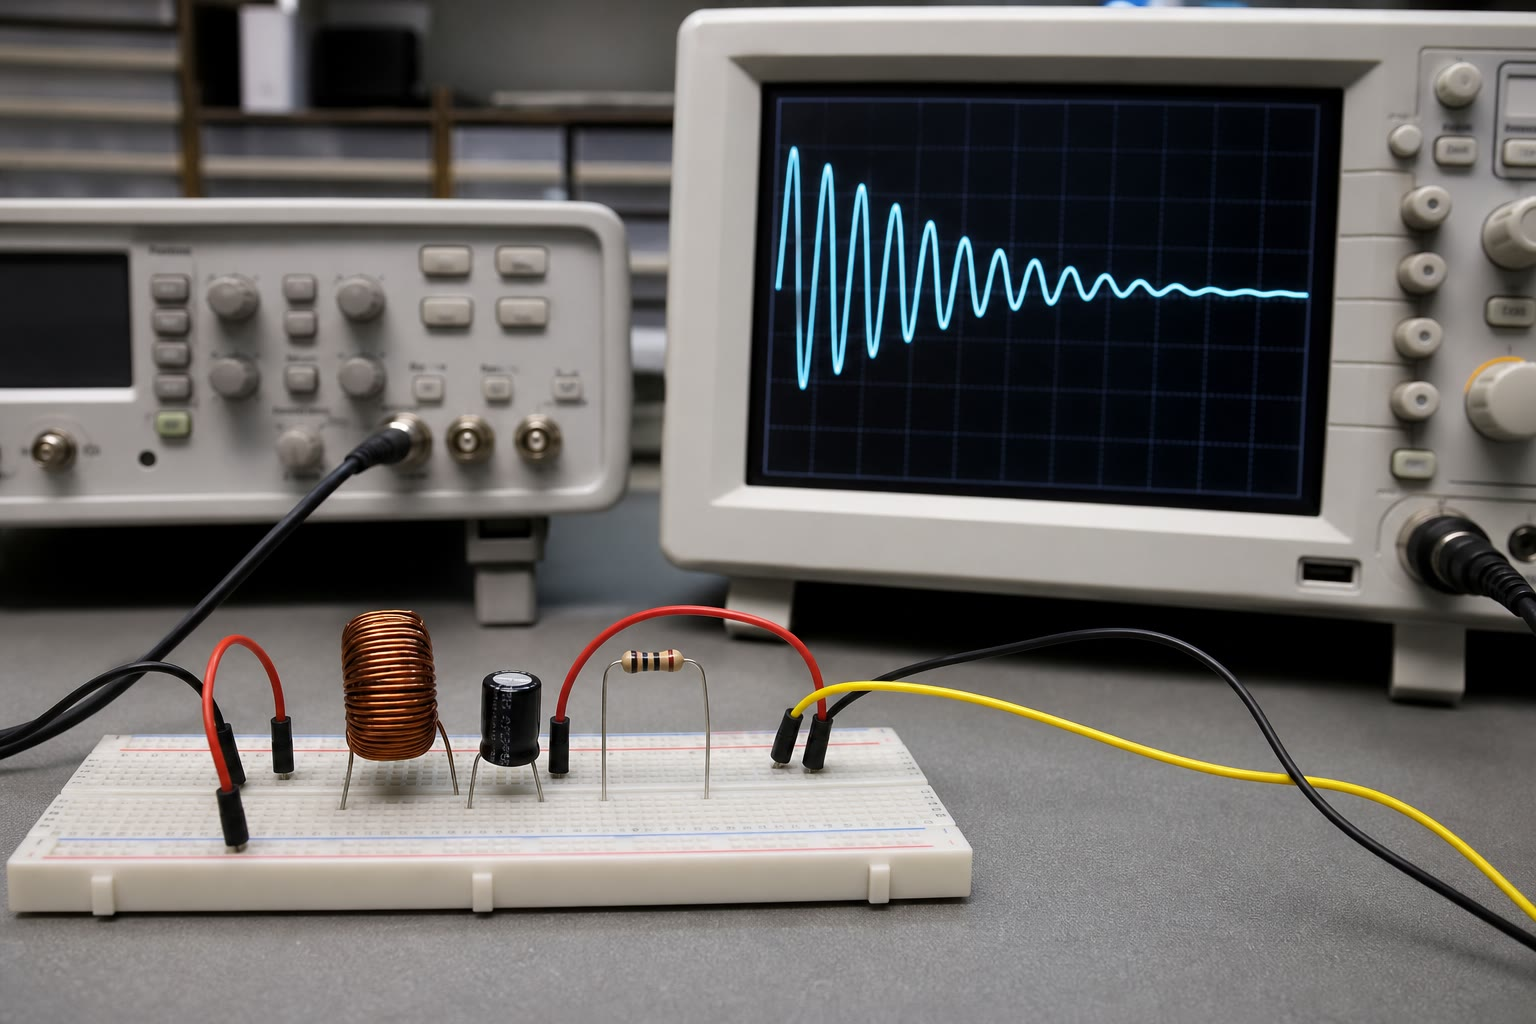
\includegraphics[width=0.60\linewidth]{images/book3/ai/b3-07-rlc-breadboard-oscilloscope.jpg}

{\small Uma bobina, um capacitor e um \omterm{def:b1:dc-circuits:resistor}{resistor} num protoboard e, no osciloscópio, a oscilação amortecida que segue um degrau: o \omterm{thm:b1:transient-regimes:regimes}{regime pseudoperiódico} deste capítulo.}
\end{omfigure}

\section{Sistemas de primeira ordem}

\begin{definition}[Sistema linear de primeira ordem]\label{def:b1:transient-regimes:firstorder}
\index{sistema de primeira ordem}\index{constante de tempo}\index{regime transitório}\index{regime permanente}
Uma grandeza $x(t)$ obedece a uma \emph{equação linear de primeira ordem com
coeficientes constantes} quando
\[
\tau\,\frac{\dd x}{\dd t} + x = x_\infty ,
\]
com $\tau > 0$ a \emph{constante de tempo} e $x_\infty$ uma constante (o
valor imposto pela fonte). O seu \emph{regime permanente} é $x = x_\infty$;
o \emph{regime transitório} é a aproximação a ele a partir do valor
inicial $x(0) = x_0$.
\end{definition}

\begin{theorem}[Solução]\label{thm:b1:transient-regimes:firstorder}
A única solução com $x(0) = x_0$ é
\[
x(t) = x_\infty + (x_0 - x_\infty)\,\eu^{-t/\tau} .
\]
A distância ao \omterm{def:b1:transient-regimes:firstorder}{regime permanente} encolhe pelo fator $\eu^{-1} \approx
0.37$ a cada $\tau$: $63\%$ do caminho em $\tau$, $95\%$ em $3\tau$,
$99\%$ em $4.6\tau$. A tangente na origem atinge $x_\infty$ em
$t = \tau$.
\end{theorem}

\begin{proof}
$y = x - x_\infty$ obedece a $\tau y' + y = 0$, cujas soluções são
$y = K\eu^{-t/\tau}$ (o curso de matemática sobre equações diferenciais
lineares mostra que não há outras); $K = x_0 - x_\infty$. A inclinação
em $0$ vale $-(x_0 - x_\infty)/\tau$, que fecharia a distância no tempo
$\tau$.
\end{proof}

\begin{omfigure}
\begin{tikzpicture}
\begin{axis}[omaxis, width=9.4cm, height=5.4cm, xlabel={$t$}, ylabel={$x$},
    xmin=0, xmax=5, ymin=0, ymax=1.35, xtick={1,2,3,4,5},
    xticklabels={$\tau$,$2\tau$,$3\tau$,$4\tau$,$5\tau$},
    ytick={0.632,1}, yticklabels={$0.63$,$x_\infty$}]
  \addplot[omExo, dashed, domain=0:5, samples=2] {1};
  \addplot[omExo, dashed, domain=0:1, samples=2] {x};
  \addplot[omDef, thick, domain=0:5, samples=100] {1 - exp(-x)};
  \draw[dashed, omExo] (axis cs:1,0) -- (axis cs:1,0.632) -- (axis cs:0,0.632);
  \draw[dashed, omExo] (axis cs:3,0) -- (axis cs:3,0.95);
  \node[omExo, below right, font=\footnotesize] at (axis cs:3,0.95) {$0.95\,x_\infty$};
  \node[omDef, font=\footnotesize, below right] at (axis cs:2.2,0.75) {$x_\infty(1 - \eu^{-t/\tau})$};
\end{axis}
\end{tikzpicture}

{\small A resposta ao degrau de primeira ordem a partir de $x_0 = 0$: a tangente
inicial encontra a assíntota em $t = \tau$; $63\%$ do caminho em $\tau$,
$95\%$ em $3\tau$. Todo transitório de primeira ordem é essa curva, dilatada
por $\tau$ e deslocada por $x_0$ e $x_\infty$.}
\end{omfigure}

\begin{proposition}[Circuitos RC e RL]\label{prop:b1:transient-regimes:rcrl}
\index{circuito RC}\index{circuito RL}
Um capacitor $C$ carregado através de um \omterm{def:b1:dc-circuits:resistor}{resistor} $R$ por uma fonte ideal $E$
obedece a $RC\,\dd u_C/\dd t + u_C = E$: $\tau = RC$, $u_{C,\infty} = E$. Uma
bobina $L$ em série com $R$ sob $E$ obedece a $(L/R)\,\dd i/\dd t + i =
E/R$: $\tau = L/R$, $i_\infty = E/R$. Retirada a fonte
($E \to 0$), as mesmas equações descrevem a descarga rumo a zero.
\end{proposition}

\begin{proof}
\omterm{thm:b1:dc-circuits:kirchhoff}{Lei das malhas} $E = Ri + u_C$ com $i = C\,\dd u_C/\dd t$; \omterm{thm:b1:dc-circuits:kirchhoff}{lei das malhas}
$E = Ri + L\,\dd i/\dd t$.
\end{proof}

\begin{proposition}[Condições de continuidade]\label{prop:b1:transient-regimes:continuity}
\index{continuidade (de $u_C$, de $i_L$)}
A \omterm{def:b1:dc-circuits:voltage}{tensão} nos terminais de um capacitor e a corrente através de um indutor são
funções contínuas do tempo: num instante de comutação $t_0$,
$u_C(t_0^+) = u_C(t_0^-)$ e $i_L(t_0^+) = i_L(t_0^-)$. As correntes nos
\omterm{def:b1:dc-circuits:resistor}{resistores} e as tensões nas bobinas podem saltar.
\end{proposition}

\begin{proof}
Um salto de $u_C$ exigiria $i = C\,\dd u_C/\dd t$ infinita, e um salto
de $i_L$ exigiria $u = L\,\dd i/\dd t$ infinita; ambos são
impossíveis num circuito de tensões e correntes finitas (de modo equivalente,
as energias armazenadas $\tfrac12 Cu_C^2$ e $\tfrac12 Li^2$ não podem mudar
instantaneamente sem potência infinita).
\end{proof}

\begin{method}[Resolvendo um transitório de primeira ordem]\label{met:b1:transient-regimes:first}
\begin{enumerate}
  \item Escreva as \omterm{thm:b1:dc-circuits:kirchhoff}{leis das malhas} e dos nós depois da comutação, com as
        leis dos componentes; reduza a uma única equação em $u_C$ ou $i_L$ e
        coloque-a na forma $\tau x' + x = x_\infty$; leia $\tau$ e
        $x_\infty$ (este último é também o \omterm{def:b1:transient-regimes:firstorder}{regime permanente} obtido
        substituindo $C$ por um circuito aberto e $L$ por um fio).
  \item Encontre $x_0$ pela continuidade de $u_C$ ou de $i_L$ através do
        instante de comutação, usando o circuito \emph{anterior} a ele.
  \item Escreva $x = x_\infty + (x_0 - x_\infty)\eu^{-t/\tau}$; deduza
        as demais grandezas por derivação e pela \omterm{thm:b1:dc-circuits:kirchhoff}{lei das malhas}.
\end{enumerate}
Quando o capacitor enxerga uma rede de \omterm{def:b1:dc-circuits:resistor}{resistores} e fontes, substitua
primeiro essa rede pelo seu equivalente de Thévenin $(E_{\mathrm{Th}}, R_{\mathrm{Th}})$
(\cref{ch:b1:dc-circuits}): $\tau = R_{\mathrm{Th}}C$,
$u_\infty = E_{\mathrm{Th}}$.
\end{method}

\begin{proposition}[Balanço energético da carga de um RC]\label{prop:b1:transient-regimes:rcenergy}
Ao carregar um capacitor de $0$ até $E$ através de um \omterm{def:b1:dc-circuits:resistor}{resistor} $R$ qualquer, a
fonte fornece $CE^2$, o capacitor armazena $\tfrac12 CE^2$ e o
\omterm{def:b1:dc-circuits:resistor}{resistor} dissipa o outro $\tfrac12 CE^2$ --- seja qual for $R$.
\end{proposition}

\begin{proof}
$i = (E/R)\eu^{-t/\tau}$; a fonte fornece $\int_0^\infty Ei\,\dd t
= E \cdot (E/R)\tau = CE^2$; o \omterm{def:b1:dc-circuits:resistor}{resistor} toma $\int_0^\infty Ri^2\,\dd t
= (E^2/R)\int_0^\infty \eu^{-2t/\tau}\dd t = (E^2/R)(\tau/2) = \tfrac12 CE^2$;
a diferença é o $\tfrac12 CE^2$ armazenado. Um $R$ menor dissipa
a mesma energia mais depressa.
\end{proof}

\begin{example}[A bobina de um relé]\label{ex:b1:transient-regimes:relay}
$L = \qty{20}{mH}$, $R = \qty{5.0}{\ohm}$, $E = \qty{10}{V}$: $\tau =
\qty{4.0}{ms}$, $i_\infty = \qty{2.0}{A}$; os contatos fecham quando
$i$ atinge \qty{1.5}{A}, isto é,\ em $t = -\tau\ln(1 - 0.75) =
\qty{5.5}{ms}$. Ao abrir o circuito, $i$ deve cair de \qty{2}{A}; um
diodo ``de roda livre'' em paralelo com a bobina lhe dá um caminho apenas
através de $R$, $\tau = \qty{4}{ms}$, em vez de uma faísca.
\end{example}

\section{Sistemas de segunda ordem}

\begin{definition}[Forma canônica de segunda ordem]\label{def:b1:transient-regimes:secondorder}
\index{sistema de segunda ordem}\index{frequência angular própria}\index{fator de qualidade}\index{fator de amortecimento}
Uma grandeza $x(t)$ é um \emph{sistema linear de segunda ordem} quando
\[
\frac{\dd^2 x}{\dd t^2} + \frac{\omega_0}{Q}\,\frac{\dd x}{\dd t} + \omega_0^2\,x
= \omega_0^2\,x_\infty ,
\]
com $\omega_0 > 0$ a \emph{\omterm{def:b1:wave-propagation:signal}{frequência angular} própria}, $Q > 0$ o
\emph{fator de qualidade} (\omterm{def:b1:units-dimensions:dimension}{adimensional}) e $x_\infty$ o \omterm{def:b1:transient-regimes:firstorder}{regime permanente}.
Escreve-se também $\omega_0/Q = 2\xi\omega_0$, com $\xi = 1/2Q$ o
\emph{fator de amortecimento}.
\end{definition}

\begin{proposition}[O circuito RLC série]\label{prop:b1:transient-regimes:rlc}
\index{circuito RLC}
Um capacitor $C$, uma bobina $L$ e um \omterm{def:b1:dc-circuits:resistor}{resistor} $R$ em série sob uma fonte
$E$: a \omterm{def:b1:dc-circuits:voltage}{tensão} do capacitor obedece à forma canônica com
\[
\omega_0 = \frac{1}{\sqrt{LC}}, \qquad Q = \frac{1}{R}\sqrt{\frac{L}{C}},
\qquad u_{C,\infty} = E .
\]
\end{proposition}

\begin{proof}
\omterm{thm:b1:dc-circuits:kirchhoff}{Lei das malhas}: $E = L\,\dd i/\dd t + Ri + u_C$ com $i = C\,\dd u_C/\dd t$:
$LC\,u_C'' + RC\,u_C' + u_C = E$; divida por $LC$ e identifique
$\omega_0^2 = 1/LC$, $\omega_0/Q = R/L$.
\end{proof}

\begin{omfigure}
\begin{tikzpicture}[font=\small]
  \draw (0,0) to[battery1, l=$E$, invert] (0,2.6) to[R=$R$] (2.4,2.6) to[L=$L$, i=$i$] (4.8,2.6) -- (4.8,2.6) to[C=$C$, v=$u_C$] (4.8,0) -- (0,0);
  \begin{scope}[xshift=7.6cm]
    \draw[thick] (0,0) -- (0,3.4);
    \fill[pattern=north east lines] (-0.25,0) rectangle (0,3.4);
    % spring
    \draw[thick] (0,2.6) -- (0.4,2.6) \foreach \i in {0,...,5} {-- ++(0.2,0.25) -- ++(0.2,-0.5) -- ++(0.2,0.25)} -- (3.3,2.6);
    % damper
    \draw[thick] (0,0.8) -- (1.2,0.8);
    \draw[thick] (1.2,0.5) -- (1.2,1.1) -- (2.2,1.1); \draw[thick] (1.2,0.5) -- (2.2,0.5);
    \draw[thick] (1.9,0.6) -- (1.9,1.0); \draw[thick] (1.9,0.8) -- (3.3,0.8);
    \draw[thick, fill=omDef!15] (3.3,0.2) rectangle (4.5,3.2); \node at (3.9,1.7) {$m$};
    \draw[-Stealth] (3.9,3.5) -- (5.2,3.5) node[right] {$x$};
    \node at (1.7,3.15) {$k$}; \node at (1.7,0.1) {$\alpha$};
  \end{scope}
\end{tikzpicture}

{\small As duas faces do \omterm{def:b1:transient-regimes:secondorder}{sistema de segunda ordem}: o \omterm{prop:b1:transient-regimes:rlc}{circuito RLC}
série ($\omega_0 = 1/\sqrt{LC}$, $Q = \sqrt{L/C}/R$) e o
conjunto massa--mola--amortecedor ($\omega_0 = \sqrt{k/m}$, $Q = \sqrt{km}/\alpha$).
Mesma equação, mesmos três regimes.}
\end{omfigure}

\begin{proposition}[O oscilador mecânico]\label{prop:b1:transient-regimes:mechanical}
\index{massa--mola--amortecedor}\index{analogia eletromecânica}
Uma massa $m$ sobre uma mola de rigidez $k$ com um amortecedor viscoso de
coeficiente $\alpha$ (força $-\alpha\dot x$), deslocada de $x$ em relação ao
equilíbrio, obedece a $m\ddot x + \alpha\dot x + kx = 0$: a forma canônica
com
\[
\omega_0 = \sqrt{\frac{k}{m}}, \qquad Q = \frac{\sqrt{km}}{\alpha} .
\]
A correspondência $x \leftrightarrow q$, $\dot x \leftrightarrow i$,
$m \leftrightarrow L$, $\alpha \leftrightarrow R$, $k \leftrightarrow 1/C$
leva todo resultado de um sistema no outro.
\end{proposition}

\begin{proof}
A segunda lei de Newton (\cref{ch:b1:newton-dynamics}) com a força da mola
$-kx$ e a força de amortecimento; divida por $m$.
\end{proof}

\begin{theorem}[Os três regimes]\label{thm:b1:transient-regimes:regimes}
\index{regime aperiódico}\index{regime crítico}\index{regime pseudoperiódico}\index{pseudoperíodo}
As soluções da equação homogênea $x'' + (\omega_0/Q)x' +
\omega_0^2 x = 0$ são governadas pelas raízes de $r^2 + (\omega_0/Q)r +
\omega_0^2 = 0$, de discriminante $\Delta = \omega_0^2(1/Q^2 - 4)$:
\begin{itemize}
  \item $Q < \tfrac12$, regime \emph{aperiódico}: duas raízes reais negativas
        $r_\pm = -\frac{\omega_0}{2Q}\big(1 \mp \sqrt{1 - 4Q^2}\big)$,
        $x = A\eu^{r_+t} + B\eu^{r_-t}$, um retorno sem oscilação;
  \item $Q = \tfrac12$, regime \emph{crítico}: uma raiz dupla $r = -\omega_0$,
        $x = (A + Bt)\eu^{-\omega_0 t}$, o retorno mais rápido sem
        ultrapassagem;
  \item $Q > \tfrac12$, regime \emph{pseudoperiódico}: raízes complexas
        $r = -1/\tau \pm \iu\omega$ com
        \[
        \tau = \frac{2Q}{\omega_0}, \qquad
        \omega = \omega_0\sqrt{1 - \frac{1}{4Q^2}},
        \qquad
        x = \eu^{-t/\tau}\big(A\cos\omega t + B\sin\omega t\big),
        \]
        uma oscilação amortecida de \emph{pseudoperíodo} $T = 2\pi/\omega$
        dentro da envoltória $\pm\sqrt{A^2 + B^2}\,\eu^{-t/\tau}$.
\end{itemize}
A solução completa com segundo membro constante é $x_\infty$ mais a
solução homogênea; $A$ e $B$ decorrem de $x(0)$ e $x'(0)$.
\end{theorem}

\begin{proof}
Equação característica de uma equação linear com coeficientes
constantes (curso de matemática, equações lineares de segunda ordem): as
raízes são $r = -\omega_0/2Q \pm \tfrac12\sqrt\Delta$. Para $Q > \tfrac12$,
$\sqrt\Delta = \iu\omega_0\sqrt{4 - 1/Q^2}$, o que dá a parte real
$-\omega_0/2Q = -1/\tau$ e a parte imaginária $\pm\omega_0\sqrt{1 - 1/4Q^2}$;
as soluções reais são as combinações de $\eu^{-t/\tau}\cos\omega t$
e $\eu^{-t/\tau}\sin\omega t$.
\end{proof}

\begin{omfigure}
\begin{tikzpicture}
\begin{axis}[omaxis, width=11.5cm, height=6cm, xlabel={$\omega_0 t$}, ylabel={$x/x_\infty$},
    xmin=0, xmax=16, ymin=0, ymax=1.75, xtick={0,5,10,15}, ytick={0.5,1,1.5},
    legend style={at={(0.97,0.97)}, anchor=north east, font=\footnotesize, draw=none, fill=none}]
  % Q=0.2: roots r = -(1/(2Q))(1 -/+ sqrt(1-4Q^2)) = -2.5(1 -/+ 0.6) = -1, -4 ; x = 1 - (4 e^{-t} - e^{-4t})/3
  \addplot[omProp, thick, domain=0:16, samples=200] {1 - (4*exp(-x) - exp(-4*x))/3};
  \addlegendentry{$Q = 0.2$ (aperiódico)}
  \addplot[omThm, thick, domain=0:16, samples=200] {1 - (1 + x)*exp(-x)};
  \addlegendentry{$Q = 0.5$ (crítico)}
  % Q=3: tau=6, w = sqrt(1-1/36)=0.986 ; x = 1 - e^{-t/6}(cos wt + sin wt /(6 w))
  \addplot[omDef, thick, domain=0:16, samples=400] {1 - exp(-x/6)*(cos(deg(0.986*x)) + sin(deg(0.986*x))/(6*0.986))};
  \addlegendentry{$Q = 3$ (pseudoperiódico)}
  \addplot[omExo, dashed, domain=0:16, samples=2] {1};
\end{axis}
\end{tikzpicture}

{\small Resposta ao degrau de um \omterm{def:b1:transient-regimes:secondorder}{sistema de segunda ordem} a partir do repouso, para três
\omterm{def:b1:transient-regimes:secondorder}{fatores de qualidade}. $Q$ pequeno: uma subida lenta; $Q = \tfrac12$: o retorno
mais rápido sem ultrapassagem; $Q$ grande: uma oscilação que dura cerca de $Q$
períodos.}
\end{omfigure}

\begin{proposition}[Lendo $Q$ num traçado pseudoperiódico]\label{prop:b1:transient-regimes:decrement}
\index{decremento logarítmico}
No \omterm{thm:b1:transient-regimes:regimes}{regime pseudoperiódico}, dois máximos sucessivos estão na razão
$x_{n+1}/x_n = \eu^{-T/\tau}$; o \emph{\omterm{prop:b1:transient-regimes:decrement}{decremento logarítmico}}
\[
\delta = \ln\frac{x_n}{x_{n+1}} = \frac{T}{\tau} = \frac{\pi}{Q\sqrt{1 - 1/4Q^2}}
\approx \frac{\pi}{Q} \quad (Q \gg 1)
\]
dá $Q$; o número de oscilações visíveis antes que a \omterm{def:b1:wave-propagation:signal}{amplitude}
caia abaixo de $5\%$ é da ordem de $Q$. Para $Q \gg 1$, $\omega \approx \omega_0$
e $T \approx 2\pi/\omega_0$.
\end{proposition}

\begin{proof}
A envoltória $\eu^{-t/\tau}$ é multiplicada por $\eu^{-T/\tau}$ a cada período;
$T/\tau = (2\pi/\omega)(\omega_0/2Q)$. A envoltória atinge $\eu^{-3}
\approx 5\%$ em $3\tau = 6Q/\omega_0 \approx Q\,T$, isto é,\ após cerca de
$Q$ períodos.
\end{proof}

\begin{omfigure}
\begin{tikzpicture}
\begin{axis}[omaxis, width=11.5cm, height=5.6cm, xlabel={$t$}, ylabel={$x$},
    xmin=0, xmax=12.5, ymin=-1.2, ymax=1.3, xtick={2,4,6,8,10,12},
    xticklabels={$T$,$2T$,$3T$,$4T$,$5T$,$6T$}, ytick={-1,1}, yticklabels={$-x_0$,$x_0$}]
  \addplot[omExo, dashed, domain=0:12.5, samples=60] {exp(-x/5)};
  \addplot[omExo, dashed, domain=0:12.5, samples=60] {-exp(-x/5)};
  \addplot[omDef, thick, domain=0:12.5, samples=500] {exp(-x/5)*cos(deg(pi*x))};
  \fill[omThm] (axis cs:0,1) circle (1.4pt) node[above right, font=\footnotesize] {$x_0$};
  \fill[omThm] (axis cs:2,0.670) circle (1.4pt) node[above right, xshift=2pt, yshift=3pt, font=\footnotesize] {$x_1 = x_0\eu^{-T/\tau}$};
  \fill[omThm] (axis cs:4,0.449) circle (1.4pt) node[above right, xshift=2pt, yshift=3pt, font=\footnotesize] {$x_2$};
\end{axis}
\end{tikzpicture}

{\small Decaimento pseudoperiódico livre, $x = x_0\eu^{-t/\tau}\cos\omega t$:
os máximos sucessivos encolhem pelo fator constante $\eu^{-T/\tau}$, e
$\ln(x_n/x_{n+1}) = T/\tau \approx \pi/Q$ mede o \omterm{def:b1:transient-regimes:secondorder}{fator de qualidade}
a partir do traçado.}
\end{omfigure}

\begin{example}[Uma oscilação RLC]\label{ex:b1:transient-regimes:rlcnum}
$L = \qty{10}{mH}$, $C = \qty{100}{nF}$, $R = \qty{100}{\ohm}$:
$\omega_0 = 1/\sqrt{10^{-9}} = \qty{3.16e4}{rad/s}$ ($f_0 =
\qty{5.03}{kHz}$), $Q = \sqrt{L/C}/R = 316/100 = 3.16$: pseudoperiódico,
$\tau = 2Q/\omega_0 = \qty{0.20}{ms}$, $\omega = 0.987\,\omega_0$,
$T = \qty{0.20}{ms}$, três oscilações visíveis. A resistência crítica
vale $R_c = 2\sqrt{L/C} = \qty{632}{\ohm}$; acima dela a descarga é
aperiódica.
\end{example}

\begin{method}[Resolvendo um transitório de segunda ordem]\label{met:b1:transient-regimes:second}
\begin{enumerate}
  \item Escreva a equação; ponha-a na forma canônica; leia $\omega_0$,
        $Q$ e $x_\infty$.
  \item Decida o regime a partir de $Q$ e escreva a solução geral como
        $x_\infty$ mais a solução homogênea.
  \item Encontre $x(0)$ e $x'(0)$ pela continuidade de $u_C$ e de $i_L$
        (para o RLC: $u_C(0^+) = u_C(0^-)$ e $u_C'(0^+) = i(0^-)/C$);
        determine as duas constantes.
\end{enumerate}
\end{method}

\begin{example}[Condições iniciais]\label{ex:b1:transient-regimes:ic}
O capacitor do exemplo anterior é carregado a $U_0$ e, em
$t = 0$, fechado sobre $L$ e $R$ (sem fonte): $x_\infty = 0$,
$u_C(0) = U_0$, $u_C'(0) = i(0)/C = 0$, pois a corrente na bobina era nula.
Logo $A = U_0$ e $-A/\tau + B\omega = 0$, $B = U_0/(\omega\tau) =
U_0/\sqrt{4Q^2 - 1}$: $u_C = U_0\eu^{-t/\tau}[\cos\omega t + \sin(\omega
t)/\sqrt{4Q^2 - 1}]$ --- para $Q \gg 1$, simplesmente $U_0\eu^{-t/\tau}\cos\omega_0 t$,
e a corrente $i = -C\,\dd u_C/\dd t$ tem pico próximo de $U_0\sqrt{C/L} =
U_0/(\omega_0 L)$.
\end{example}

\begin{remark}[Energia]\label{rem:b1:transient-regimes:energy}
A energia armazenada $\tfrac12 Cu_C^2 + \tfrac12 Li^2$ (ou $\tfrac12 kx^2
+ \tfrac12 m\dot x^2$) decresce à taxa $Ri^2$ ($\alpha\dot x^2$):
derive e use a equação. A cada pseudoperíodo a energia
encolhe pelo fator $\eu^{-2T/\tau}$; com $Q = 3$, cerca de $88\%$ dela
se perde por oscilação. Um $Q$ alto significa um vazamento lento em relação à
oscilação --- um bom relógio, uma ressonância aguda
(\cref{ch:b1:sinusoidal-impedance}) --- e um $Q$ baixo, um retorno rápido:
a escolha certa para uma suspensão ou para o ponteiro de um instrumento.
\end{remark}

\section{Exercícios}

\begin{exercise}[$\star$]\label{exo:b1:transient-regimes:1}
Um \omterm{prop:b1:transient-regimes:rcrl}{circuito RC}: $R = \qty{10}{k\ohm}$, $C = \qty{47}{nF}$, carregado a partir de
$E$. Calcule $\tau$, $u_C(\tau)/E$ e o tempo para atingir $99\%$ de $E$.
\end{exercise}

\begin{exercise}[$\star$]\label{exo:b1:transient-regimes:2}
Um \omterm{prop:b1:transient-regimes:rcrl}{circuito RL}: $L = \qty{20}{mH}$, $R = \qty{5.0}{\ohm}$, $E = \qty{10}{V}$.
Calcule $\tau$, a corrente final, a corrente em $t = \tau$ e a
\omterm{def:b1:dc-circuits:voltage}{tensão} na bobina logo após o fechamento da chave.
\end{exercise}

\begin{exercise}[$\star$]\label{exo:b1:transient-regimes:3}
Um RLC série: $L = \qty{10}{mH}$, $C = \qty{100}{nF}$, $R = \qty{100}{\ohm}$.
Calcule $\omega_0$, $f_0$, $Q$; nomeie o regime; dê $\tau$ e o
pseudoperíodo.
\end{exercise}

\begin{exercise}[$\star$]\label{exo:b1:transient-regimes:4}
Com os mesmos $L$ e $C$, que resistência dá o \omterm{thm:b1:transient-regimes:regimes}{regime crítico}?
Quanto vale $Q$ nesse caso? O que acontece para $R = \qty{2}{k\ohm}$?
\end{exercise}

\begin{exercise}[$\star\star$]\label{exo:b1:transient-regimes:5}
Um capacitor carregado $C = \qty{1.0}{\micro F}$ se descarrega através de um
$R$ desconhecido; a \omterm{def:b1:dc-circuits:voltage}{tensão} cai à metade a cada \qty{3.5}{ms}. Mostre que a
meia-vida vale $\tau\ln 2$ e encontre $R$.
\end{exercise}

\begin{exercise}[$\star\star$]\label{exo:b1:transient-regimes:6}
Mostre por integração direta que carregar um capacitor de $0$ a $E$
através de $R$ dissipa exatamente $\tfrac12 CE^2$ em $R$, independentemente de
$R$. Qual é, então, o rendimento da transferência, e como se poderia
fazer melhor?
\end{exercise}

\begin{exercise}[$\star\star$]\label{exo:b1:transient-regimes:7}
Num osciloscópio, um decaimento RLC livre mostra máximos sucessivos de
\qty{2.0}{V}, \qty{1.5}{V}, \qty{1.12}{V} a intervalos de \qty{0.40}{ms}.
Deduza $Q$, $\omega_0$ e, com $C = \qty{1.0}{\micro F}$, os valores
de $L$ e de $R$.
\end{exercise}

\begin{exercise}[$\star\star$]\label{exo:b1:transient-regimes:8}
Um capacitor carregado a $U_0 = \qty{100}{V}$ ($C = \qty{10}{\micro F}$) é
comutado sobre uma bobina $L = \qty{1.0}{mH}$ de resistência pequena ($Q \gg 1$).
Escreva $u_C(t)$ e $i(t)$ e estime a corrente de pico. Onde está
a energia no pico?
\end{exercise}

\begin{exercise}[$\star\star$]\label{exo:b1:transient-regimes:9}
Um quarto de carro: $m = \qty{400}{kg}$ sobre uma mola $k = \qty{2.0e4}{N/m}$.
Calcule $\omega_0$, $f_0$ e o coeficiente de amortecimento crítico. Com um
amortecedor $\alpha = \qty{2000}{N.s/m}$, dê $Q$, o regime, o
pseudoperíodo e o tempo de decaimento $\tau$.
\end{exercise}

\begin{exercise}[$\star\star\star$]\label{exo:b1:transient-regimes:10}
Uma bobina $L = \qty{0.50}{H}$ conduz $I_0 = \qty{2.0}{A}$; a fonte é
desligada e a bobina fica ligada a um \omterm{def:b1:dc-circuits:resistor}{resistor} de descarga $R = \qty{100}{\ohm}$.
Dê $i(t)$, $\tau$, a \omterm{def:b1:dc-circuits:voltage}{tensão} de pico na bobina e a energia
dissipada. O que aconteceria sem o \omterm{def:b1:dc-circuits:resistor}{resistor}?
\end{exercise}

\begin{exercise}[$\star\star\star$]\label{exo:b1:transient-regimes:11}
Um capacitor $C = \qty{1.0}{\micro F}$ é carregado a partir de $E = \qty{12}{V}$
através de $R_1 = \qty{10}{k\ohm}$, com $R_2 = \qty{20}{k\ohm}$ ligado
em paralelo com ele. Usando um equivalente de Thévenin, encontre a \omterm{def:b1:transient-regimes:firstorder}{constante de tempo} e a
\omterm{def:b1:dc-circuits:voltage}{tensão} final; escreva $u_C(t)$ a partir de $u_C(0) = 0$.
\end{exercise}

\begin{exercise}[$\star\star\star$]\label{exo:b1:transient-regimes:12}
\omterm{thm:b1:transient-regimes:regimes}{Regime crítico}, degrau a partir do repouso ($x(0) = x'(0) = 0$): mostre que
$x = x_\infty[1 - (1 + \omega_0 t)\eu^{-\omega_0 t}]$ e encontre
numericamente o tempo para atingir $95\%$ de $x_\infty$ (em unidades de
$1/\omega_0$). Compare com o tempo de \omterm{def:b1:optical-instruments:eye}{acomodação} da envoltória para $Q = 5$
e com o da raiz lenta quando $Q = 0.1$; conclua por que o regime ``crítico'' é o
alvo do engenheiro.
\end{exercise}

\section{Problema: projetando uma suspensão}

\begin{problem}[{Problema de fim de semana --- a mesma equação diferencial numa
bancada de laboratório e sob um carro: quantos balanços um amortecedor gasto
permite, o que o projetista escolhe em vez disso e como um único número distingue
os dois}]
\label{pb:b1:transient-regimes:1}
A Parte I estuda um \omterm{prop:b1:transient-regimes:rlc}{circuito RLC} série, $L = \qty{10}{mH}$, $C = \qty{100}{nF}$;
as Partes II--IV, um modelo de quarto de carro: uma massa $m = \qty{350}{kg}$ apoiada numa
mola $k = \qty{22}{kN/m}$ e num amortecedor que exerce $-\alpha\dot x$.
Ultrapassagem de uma resposta ao degrau no \omterm{thm:b1:transient-regimes:regimes}{regime pseudoperiódico} (dada):
$x_{\max}/x_\infty - 1 = \exp(-\pi\xi/\sqrt{1 - \xi^2})$, $\xi = 1/2Q$.

\medskip
\noindent\textbf{Parte I --- O circuito.}
\begin{enumerate}
  \item Escreva a \omterm{thm:b1:dc-circuits:kirchhoff}{lei das malhas} para o RLC série sob uma fonte $E$ e a
        equação diferencial de $u_C$.
  \item Ponha-a na forma canônica; exprima $\omega_0$ e $Q$.
  \item Calcule $\omega_0$, $f_0$ e a resistência crítica $R_c$.
  \item Escreva a equação característica e o seu discriminante; enuncie
        os três regimes em termos de $Q$.
  \item No caso pseudoperiódico, dê $\tau$ e $\omega$ e a
        forma de $u_C(t)$.
  \item Para $R = \qty{100}{\ohm}$ calcule $Q$, $\tau$, o pseudoperíodo
        e o número de oscilações visíveis.
  \item O capacitor, carregado a $U_0$, é comutado sobre $L$ e $R$
        em $t = 0$. Dê $u_C(0^+)$ e $\dd u_C/\dd t(0^+)$, com a
        razão física de cada um.
\end{enumerate}

\medskip
\noindent\textbf{Parte II --- O quarto de carro.}
\begin{enumerate}[resume]
  \item Medindo $x$ a partir da posição de equilíbrio, escreva a segunda
        lei de Newton para a carroceria e mostre que o peso desaparece.
  \item Ponha a equação na forma canônica; dê $\omega_0$ e $Q$ em
        termos de $m$, $k$, $\alpha$, e liste as correspondências
        eletromecânicas.
  \item Calcule $\omega_0$, $f_0$ e o coeficiente crítico
        $\alpha_c$.
  \item O projetista monta $\alpha = \qty{4000}{N.s/m}$: calcule $Q$,
        $\xi$, e nomeie o regime.
  \item Calcule $\tau$ e o pseudoperíodo.
  \item Calcule a ultrapassagem após um degrau (um meio-fio): o carro é
        confortável?
  \item Que resistência $R$ daria ao circuito da Parte I o mesmo
        $Q$ desta suspensão?
\end{enumerate}

\medskip
\noindent\textbf{Parte III --- O amortecedor gasto.}
Vazou óleo: $\alpha = \qty{1200}{N.s/m}$.
\begin{enumerate}[resume]
  \item Calcule $Q$, o pseudoperíodo e $\tau$.
  \item Por qual fator os máximos sucessivos encolhem? Quantos balanços
        são visíveis antes que a \omterm{def:b1:wave-propagation:signal}{amplitude} fique abaixo de $5\%$?
  \item O teste do balanço: empurra-se o canto para baixo em $x_0 =
        \qty{5.0}{cm}$ e solta-se. Dê as condições iniciais, a
        energia armazenada na mola e diga para onde vai essa energia.
  \item Estime a velocidade de pico da carroceria durante o primeiro
        retorno ($\approx x_0\omega_0$ para $Q \gg 1$) e a força de pico
        no amortecedor.
  \item Por que o amortecimento exatamente crítico ($Q = \tfrac12$) não é a
        escolha do projetista, embora não produza ultrapassagem? (Pense nos
        últimos milímetros do retorno.)
  \item Calcule a ultrapassagem para o amortecedor gasto e compare com a
        Parte II.
\end{enumerate}

\medskip
\noindent\textbf{Parte IV --- Diagnosticando $Q$ num traçado.}
Um acelerômetro na carroceria registra o decaimento livre.
\begin{enumerate}[resume]
  \item Para o carro gasto, os máximos sucessivos valem $1.00$, $0.25$, $0.062$
        (unidades arbitrárias). Calcule o \omterm{prop:b1:transient-regimes:decrement}{decremento logarítmico}, deduza
        $\xi$ exatamente de $\delta = 2\pi\xi/\sqrt{1 - \xi^2}$ e depois $Q$;
        compare com a Parte III.
  \item Para o carro em bom estado nenhum segundo máximo é visível; só a
        ultrapassagem, $3.8\%$, pode ser lida. Inverta a fórmula da ultrapassagem para
        encontrar $\xi$ e $Q$.
  \item Que fração da energia mecânica o amortecedor gasto
        dissipa por pseudoperíodo?
  \item Um técnico que não tem um carro à mão monta o RLC da Parte I
        com $R$ escolhido de modo que $Q = 2.3$: que $R$, e por que o
        traçado do osciloscópio, plotado contra $\omega_0 t$, tem forma idêntica
        à do carro?
  \item Resuma: que número \omterm{def:b1:units-dimensions:dimension}{adimensional} decide a forma de qualquer
        transitório de segunda ordem, que valor um projetista de suspensão
        busca e o que um motorista deve concluir de ``mais de um
        balanço''.
\end{enumerate}
\end{problem}
